% !TeX root = ../../thesis.tex
\chapter{Discussion}\label{ch:discussion}

\begin{minipage}[b]{0.65\textwidth}
    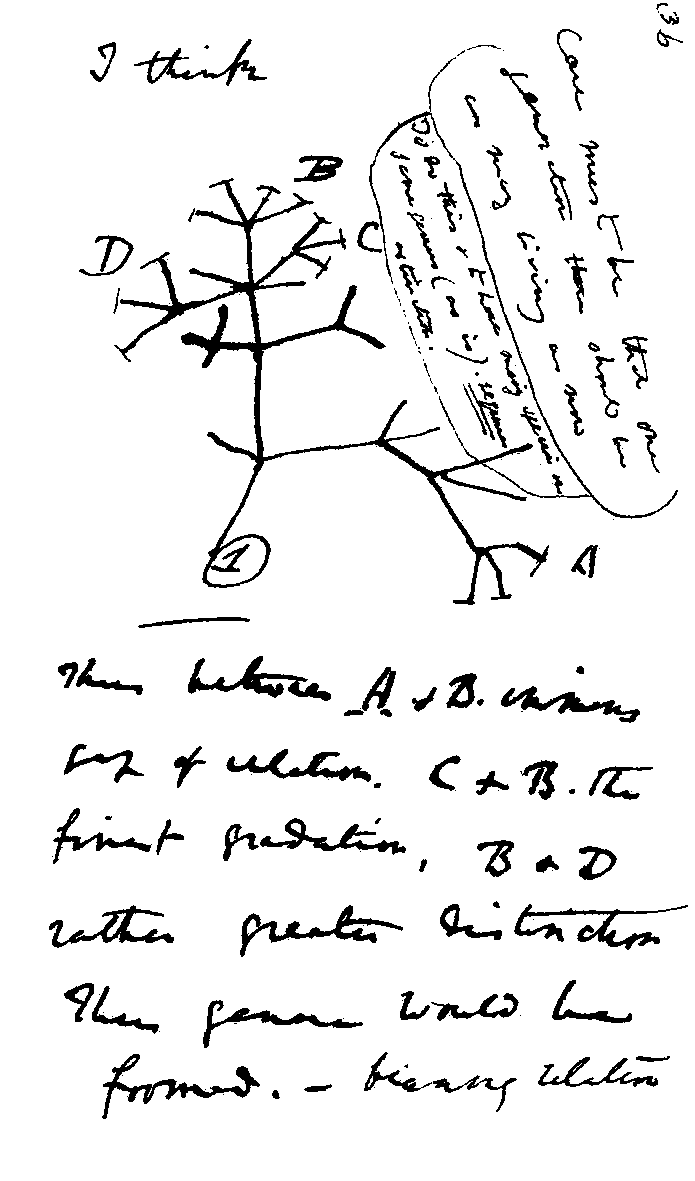
\includegraphics[width=\textwidth]{title} % Note: image needs to be cropped and faded
  \end{minipage}
  \hfill
  \begin{minipage}[b]{0.35\textwidth}
    \footnotesize
    \begin{flushright}
      \textit{``\ldots a tiny twig\\on an improbable branch\\of a contingent limb\\on a fortunate tree.''} \\
      --- Stephen Jay Gould
    \end{flushright}
    \vspace{2cm}
  \end{minipage}

\clearpage

\onehalfspacing

\section{Genomic epidemiology across time scales}
In this PhD thesis we have explored the application of phylodynamic methods to understand viral spread and evolution across three distinct temporal scales, demonstrating both the versatility and limitations of genomic epidemiology as a tool for public health.
Through analyses ranging from real-time \gls{sarscov2} surveillance during the COVID-19 pandemic to the reconstruction of ancient hepatitis B virus spread, we showed how \textit{different temporal contexts necessitated different analytical approaches} while remaining grounded in the same fundamental phylodynamic theory.

The real-time analysis of \gls{sarscov2} in Belgium (Chapter~\ref{ch:chapter1}) demonstrated the power of rapid phylodynamic inference to inform ongoing public health responses, despite computational and methodological constraints.
This work highlighted both the potential and challenges of integrating genomic surveillance into routine public health practice, requiring a careful balance between analytical thoroughness and the need for timely results.
The post hoc analysis of BA.1 (Omicron) emergence in Pakistan (Chapter~\ref{ch:chapter2}) exemplified how more computationally intensive Bayesian methods could provide deeper insights into viral emergence and spread when time constraints were relaxed.
Finally, our investigation of long-term \gls{hbv} evolution (Chapter~\ref{ch:chapter3}) revealed how phylodynamic methods could reconstruct historical patterns of viral spread while simultaneously illuminating the impact of globalization on contemporary viral dynamics.

These analyses, though conducted at different time scales and employing different statistical approaches, shared common theoretical foundations and faced similar fundamental challenges.
Issues of sampling bias, computational limitations, and the integration of genomic and epidemiological data persist across all temporal scales, though their specific manifestations and solutions differ.
Together, these studies demonstrate how the field of genomic epidemiology can be used to address biological and epidemiological questions across multiple temporal scales, while also highlighting areas where methodological advancement is still needed.

\subsection{Real-time genomic epidemiology}
Our real-time analysis of \gls{sarscov2} in Belgium presented both significant challenges and valuable lessons for genomic surveillance during public health emergencies.
Initially, we encountered substantial obstacles related to data standardization and sharing practices.
Different sequencing facilities and data providers used varying formats for metadata encoding, making data integration time-consuming and error-prone.
These challenges highlighted the critical need for \textit{standardized data reporting frameworks} in outbreak scenarios, as time spent on data cleaning and reformatting directly reduced time available for analysis and reporting.

The availability of open-source tools, particularly Nextstrain, proved instrumental in overcoming these initial hurdles.
Rather than developing custom analysis pipelines from scratch, we were able to adapt existing, well-tested frameworks to our specific needs.
This approach not only accelerated our ability to begin meaningful analysis but also enhanced the reliability of our results through the use of validated, peer-reviewed software.
The experience of the Belgian genomic surveillance program was a microcosm of how \textit{free, open-source tools democratize access to phylodynamic analysis}, enabling similar surveillance efforts worldwide during the pandemic \citep{hodcroft2021spread,sahadeo2023implementation}.

We established a robust system that facilitated semi-weekly, actionable insights to the Belgian Consultative Committee throughout 2021 and 2022.
Our pipeline processed new sequence data, integrated it with existing datasets, performed phylodynamic analyses, and generated publicly available web visualizations within a 48-hour turnaround time.
The reproducibility of our workflow was particularly crucial, as it allowed us to maintain consistent analysis standards as novel variants arose, requiring us to devote minimal time to setting up new analyses as they became necessary.
Furthermore, by making our results publicly available through online platforms, we maintained transparency in our scientific process which (hopefully) engendered some amount of public trust at a time when skepticism in the scientific process was on the rise globally.

The this real-time surveillance system demonstrated the three key principles that were essential for outbreak genomic epidemiology: \textit{speed, reproducibility, and transparency}.
Speed was critical for ensuring that insights could inform public health decision-making in a timely manner.
Reproducibility enabled us to maintain consistent analysis standards even as new variants arose.
Transparency---through public sharing of both methods and results---fostered collaboration and helped build public trust in scientific findings.
As we anticipate and prepare for future viral epidemics, these principles provide a valuable framework for genomic surveillance.

\subsection{\textit{Post hoc} outbreak genomic epidemiology}
Our \textit{post hoc} analysis of BA.1 emergence in Pakistan demonstrated both the power and limitations of phylogeographic methods when applied to countries with limited genomic surveillance capacity.
Pakistan, like many lower- and middle-income countries \citep{brito2022global}, contributed relatively few sequences to GISAID compared to North American and European nations.
This sampling bias presented significant analytical challenges, requiring careful subsampling strategies to prevent over representation of highly sampled regions from obscuring true patterns of viral spread.
Additionally, the sheer size of the global BA.1 dataset necessitated substantial computational resources and time, even after subsampling.
These challenges highlighted the ongoing need for both \textit{expanded global surveillance capacity} and more \textit{efficient computational methods} for analyzing increasingly large datasets.

Despite these limitations, our analysis revealed several insights into BA.1's introduction and spread in Pakistan.
We found that the \textit{majority of BA.1 introductions into Pakistan originated from Northern Europe}, and that the majority of these introductions were linked to Pakistan's most globally connected cities.
This underscores the continued importance of air travel in driving \gls{sarscov2} spread.
Interestingly, while Pakistan received multiple BA.1 introductions, our analysis suggested that the country \textit{did not serve as a major source of onward transmission} to other regions during the early Omicron wave.
This limited onward spread was likely due to both the rapid global emergence of BA.1 and its subsequent replacement by BA.2, which occurred just a few months after BA.1's rise to local and global predominance.
These results provided valuable insights into the patterns of variant spread in Pakistan while highlighting the importance of increasing genomic surveillance capacity in countries that have been historically underrepresented.

\subsection{Paleogenomic epidemiology}
Our analysis of \gls{hbv} genotypes A, D, and E demonstrated how careful methodological choices can help overcome the challenges in reconstructing ancient viral spread patterns.
The extremely long timescale of \gls{hbv} evolution necessitated several analytical considerations.
We employed a strongly informative molecular clock prior based on previous studies \citep{kocher2021ten}, which helped constrain evolutionary rate estimates over millennia.
Our geographic partitioning scheme was designed to reflect historical human population structures rather than modern political boundaries, acknowledging that contemporary national borders would be meaningless for much of \gls{hbv}'s evolutionary history.
Perhaps most crucially, the inclusion of ancient \gls{hbv} genomes recovered from archaeological remains provided crucial calibration points, allowing us to more accurately estimate divergence times and evolutionary rates.

The resulting phylogeographic reconstruction revealed how \gls{hbv}'s spread patterns have been fundamentally driven by human movement patterns.
During most of its evolutionary history, \gls{hbv} dispersal was limited by human mobility, with spread patterns largely following the slow pace of human migration.
However, this dynamic shifted dramatically with the onset of globalization.
We observed increased viral movement coinciding with major historical events, including a notable introduction of \gls{hbv} genotype A to the Americas that coincided with the transatlantic slave trade.
In more recent decades, we found evidence of increasingly frequent viral movement between geographic regions, reflecting the impact of modern transportation networks and human mobility patterns on viral spread.

These findings have direct implications for contemporary public health practices, particularly given the relationship between \gls{hbv} genotypes and treatment outcomes.
Different \gls{hbv} genotypes show varying responses to antiviral therapies and are associated with different disease risks.
Our reconstruction of genotype-specific spread patterns helps explain current geographic distributions of \gls{hbv} diversity, which in turn can inform regional treatment strategies and public health planning.
Furthermore, understanding how globalization has accelerated viral movement helps predict how \gls{hbv} genotype distributions may continue to shift in response to changing patterns of human mobility, allowing healthcare systems to adapt their screening and treatment protocols accordingly.

\section{Future directions}
\subsection{Extensions to other pathogens and timescales}
One of the most promising future directions for phylodynamic analysis is the development of methods that would enable Bayesian inference in real-time outbreak settings.
While maximum likelihood approaches currently provide the necessary speed for immediate public health response, they lack robust methods with which to quantify uncertainty---a feature that makes Bayesian methods so valuable for understanding complex epidemiological dynamics.
Recent advances in computational methods, including Hamiltonian Monte Carlo approaches \citep{baele2020hamiltonian,ji2023scalable} and online Bayesian inference \citep{gill2020online,dinh2018online}, suggest potential pathways for achieving Bayesian inference with significantly reduced computational time.
Additionally, the development of new algorithms to exploit cutting-edge parallelized hardware could significantly reduce phylogenetic likelihood computation times---the most time consuming part of both Bayesian and ML phylogenetic inference.
Such advances would be particularly valuable during outbreak responses, allowing public health officials to better understand the uncertainty in their predictions while maintaining the rapid turnaround times necessary for actionable insights.

\subsection{Pandemic scale phylodynamics}
The scale of genomic epidemiology has been transformed by the COVID-19 pandemic, with GISAID now hosting over 20 million \gls{sarscov2} genomes---a dataset size that would have been unimaginable just five years ago.
This unprecedented scale of data generation demands new computational approaches and infrastructure to handle ``pandemic-scale'' datasets, as future outbreak responses will likely generate similarly massive datasets that must be analyzed rapidly and robustly to inform public health decision-making.

\subsubsection{New approaches to phylodynamics}
We have learned that the currently existing analytical paradigms do not always scale well with dataset size, and new approaches are being continually developed to try to keep up.
Thorney BEAST---an extension of \gls{beast} that replaces the standard phylogenetic likelihood with less computationally demanding Poisson likelihood on mutation counts \citep{thorne1998estimating}---has been used to apply Bayesian phylogenetic inference to datasets of upwards of 10\,000 taxa \citep{du2021establishment}.
Programs such as UShER \citep{turakhia2021ultrafast} and Delphy (\url{https://delphy.fathom.info/}) seek to use new tree encoding schema to reduce the computational burden of phylogenetic analysis.
Others seek to use methods such as variational inference \cite{zhang2019variational} to estimate phylogenetic posterior probability distributions using non-\gls{mcmc} methodologies.

\subsubsection{Dataset exploration and visualization}
It is perhaps obvious to state that as phylogenetic datasets grow, so do the phylogenies that relate their taxa.
Historically, many inferences drawn from phylogenetic analyses have come from methods like ``looking at the tree'' and ``counting certain features.''
With increasing dataset size, these tools prove less useful, as such tasks become onerous on trees representing even a few thousand taxa.
Consider the phylogeny from Chapter~\ref{ch:chapter2}, which relates 1\,700 taxa; the full, labeled tree (Suppl.~Fig.~\ref{sfig:fullPKTree}) spans several pages, and is incredibly difficult to parse visually.
Additionally, it is convention for papers that perform phylogenetic inference to show a tree, however this is either impossible to do, in the case of large, legible trees, or the resultant trees are nearly uninterpretable because of how much they need to be downscaled to fit the target figure size.

To handle these problems, future researchers will need to develop both standardized algorithmic tools for extracting more useful information from trees, and to establish new norms for the visual display of phylogenetic information.
New algorithms should make it easier for phylogeneticists to identify and interrogate parts of potentially massive phylogenies that may contain characteristics of public health interest, as well as to reduce some of the noise that can be presented by large background datasets.
Visual tools should then fall naturally from these algorithms, so that researchers can present more compelling, interpretable visualizations of the large phylogenies that they infer.

\section{Final remarks}
The integration of molecular techniques with traditional epidemiology has revolutionized our ability to understand and combat viral pathogens.
Through this dissertation, we have seen how genomic epidemiology can be applied across multiple timescales to address diverse public health challenges.
The COVID-19 pandemic, despite its devastating impact, catalyzed a movement of global scientific collaboration and data sharing that has transformed our capacity to respond to viral threats.

While the challenges posed by emerging infectious diseases remain significant---particularly as human expansion into natural environments increases the risk of zoonotic spillover---in the pandemic era, we possess powerful tools to detect, track, and respond to viral threats.
The continuing advancement (and subsequently decreasing cost) of sequencing technologies, coupled with increasingly sophisticated analytical methods, positions us to respond more effectively to future outbreaks.
Moreover, the establishment of global genomic surveillance networks during the COVID-19 pandemic has created sustainable infrastructure for early warning systems for other viruses of global public health concern.

The future of genomic epidemiology lies not just in technological advancement, but in maintaining and strengthening the spirit of global scientific cooperation that was fortified during the pandemic.
By sharing data, methods, and expertise across borders, we can ensure that tools for understanding viral spread and evolution remain accessible to all.
While viruses may continue to pose significant challenges to human health, our collective ability to understand and respond to these threats in a timely manner has never been stronger.

%%%%%%%%%%%%%%%%%%%%%%%%%%%%%%%%%%%%%%%%%%%%%%%%%%
% Keep the following \cleardoublepage at the end of this file,
% otherwise \includeonly includes empty pages.
\cleardoublepage

% vim: tw=70 nocindent expandtab foldmethod=marker foldmarker={{{}{,}{}}}
